\documentclass[11pt]{article}
\usepackage[margin=.8in]{geometry}
\usepackage{amsmath,amssymb,graphicx,hyperref}
\setlength{\parindent}{0pt}
\setlength{\parskip}{6pt}
\begin{document}
\begin{center}
{\Large An actual integral residual ideal is constructed}\\
23 November 2026 --- local unsigned Lean component evidence
\end{center}

\textbf{Actual result.}
Retain the actual nonsingular Weierstrass target and three opposite point-pairs,
explicit \(a_1=a_3=0\), nonzero two and ordinates, target outside the paired set,
and the original finite-operator witness construction.
The prior normalized function \(h\) is actually nonzero, has algebra-norm
degree at most six and belongs to the actual target ideal \(I^4\).
Lean now constructs an actual integral ideal \(J\) with
\[
 H=\langle h\rangle=I^4J,\qquad
 R/J\text{ finite dimensional},\qquad
 \dim_K(R/J)\le6,\quad R=K[W].
\]
No successful residual \(J\) is supplied
(PCC-20261123-cba56c) [pcc:unverified].

\begin{center}
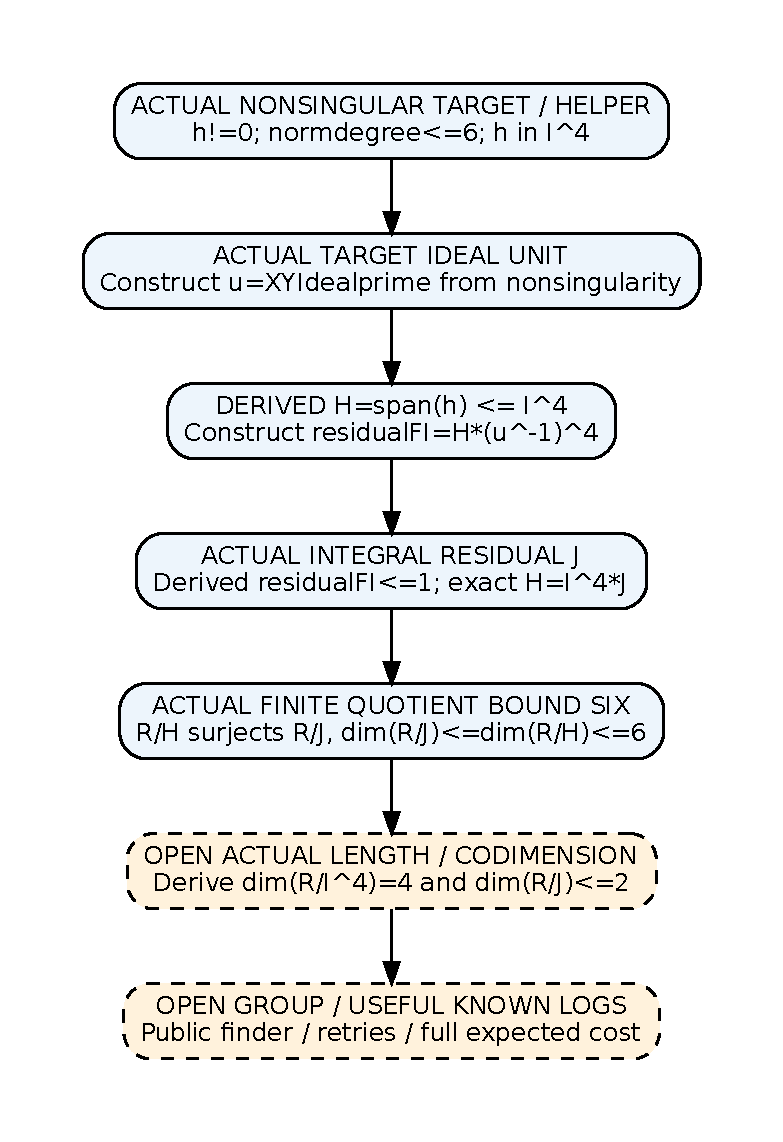
\includegraphics[height=5.0in,width=.95\linewidth,keepaspectratio]{residual-ideal-dependencies-001.pdf}
\end{center}
The solid construction is checked at the stated scope.
The bound \emph{six} is retained; the sharper bound two requires a separate
actual quotient-length argument. The diagram records implications, not
runtime or scaling measurements.

\newpage
\begin{center}{\Large Exact construction, checks and remaining dimension gap}\end{center}

\textbf{Integral factor construction.}
The actual nonsingular point supplies the public invertible fractional point
ideal \(u\) representing \(I\). Derived membership \(h\in I^4\) gives
\(H=\langle h\rangle\subseteq I^4\).
Construct the fractional residual \(J_f=H(u^{-1})^4\).
Actual order monotonicity and unit-power cancellation give \(J_f\subseteq1\).
The existing public integral criterion constructs \(J\) whose fractional image
is \(J_f\), and integral-ideal injection gives the exact equality \(H=I^4J\).
This is standard ideal/localization algebra reused; neither \(J\) nor the
factorization is an input witness [pcc:unverified].

\textbf{Finite quotient bound.}
The existing actual coordinate-ring norm theorem identifies
\(\dim_K(R/H)\) with the actual norm degree, at most six.
Since an ideal product is contained in either factor, \(H=I^4J\subseteq J\).
The actual quotient map \(R/H\to R/J\) is surjective.
It gives actual residual finiteness and
\(\dim_K(R/J)\le\dim_K(R/H)\le6\).
No subtraction by four is used or assumed [pcc:unverified].

\textbf{Proof map and standing.}
Source070/build074/local037 checks186 primary statements, four new since182:
\texttt{actual\_\allowbreak{}integral\_\allowbreak{}residual},
\texttt{actual\_\allowbreak{}principal\_\allowbreak{}quotient\_\allowbreak{}bound},
\texttt{actual\_\allowbreak{}residual\_\allowbreak{}quotient\_\allowbreak{}bound},
\texttt{actual\_\allowbreak{}residual\_\allowbreak{}witness},
in namespace \texttt{OrientationActualResidualIdeal}.
The run exits zero without warnings; all printed foundations are standard.
PCC-20261123-cba56c remains unsigned local data, outside historical shared
Transport53/57 audit/fresh [pcc:unverified].

Separate owner \texttt{CryptoLean.InvertibleIdealResidual} at
\texttt{ba07267} has focused build and unchanged actual audit:
two theorems, zero failing, zero extra trusted.
Its inspected single-page editable report and exact source/dependency hashes
are pinned. PCC-20261123-a39eba/aed40e/b1692b bind the owner stages;
only the final004 has zero warnings. Lean4.35.0 and Mathlib revision
\texttt{cfc55fc} are pinned in the receipts [pcc:unverified].

\textbf{Next discriminating obligation.}
Public Mathlib Picard results make invertible modules free of rank one over
semilocal rings. A finite-dimensional quotient algebra is Artinian and
semilocal. Derive the actual base-change linear equivalence and field dimension
from those laws without supplying a favorable basis; then identify the actual
ideal quotient and use the actual short exact sequence to obtain product
codimension additivity. The target \(I^4\) dimension four and residual dimension
two remain separate actual conclusions to establish.

Only after the degree/group bridge should the fixed known-log base coverage
be evaluated. Residual ideals or roots alone do not supply discrete logarithms.
Actual residual fields, useful known labels, public finder/coverage/retries and
complete expected bit cost remain open. The original general prime-curve
criteria are unchanged.

\textbf{Preservation.}
Rejected consumer069/build073 and owner001 API errors, owner002/003
unused-domain warnings and final004 remain exact. No linter, class, trust,
resource or private-body override was used. Prior frozen reports/sources/raw
and the exact local ledger prefix remain intact; protected canonical ledger
divergence blocks remote publication only.
\end{document}
